\documentclass[a4paper,12pt]{article}
\usepackage{amsmath}
\usepackage{cite}
\usepackage{graphicx}
\graphicspath{ {images/} }

\begin{document}
\title{DCA based Methods for Protein-Protein Interface}
\author{Linh Dang}
\date{07.04.15} 
\maketitle

\section*{DCA based Approaches for Heterodimer Proteins}
\subsection*{Problem Statement}
We examine the heterodimer protein complex where there are one big and one small protein chain. In this report, we take the protein complex with PDBID 4a0r as an example. 
\subsection*{Method}
Briefly, we use the idea of concatenated MSA to predict inter-contact between two heterodimer protein chains. In addition, DCA and Gremlin score are examined. 
\subsection*{Results}
In figures \ref{3d_gremlin} and \ref{3d_dca}, the correlation among DCA based methods score (dca and gremlin scores) and the actual distance is quite weak. Hence, it is not very reliable to use primitive dca scores to predict the contact in the interface. 
In addition, in figure \ref{dca_gremlin}, it shows that the gremlin and dca scores are relatively equivalent. 

\begin{figure}
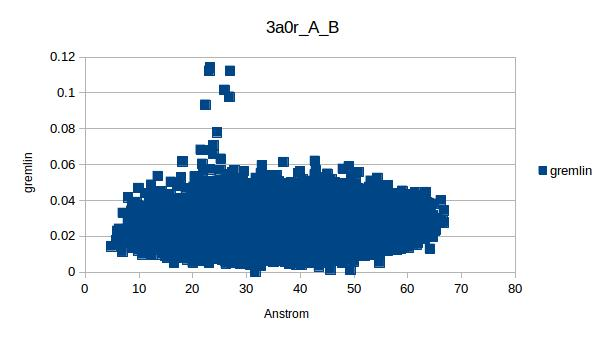
\includegraphics[scale=0.4]{3a0r_AB_3d_gremlin.jpg}
\caption{X axis: 3D distance in Anstrom. Y axis: Gremlin score}
\label{3d_gremlin}
\end{figure}

\begin{figure}
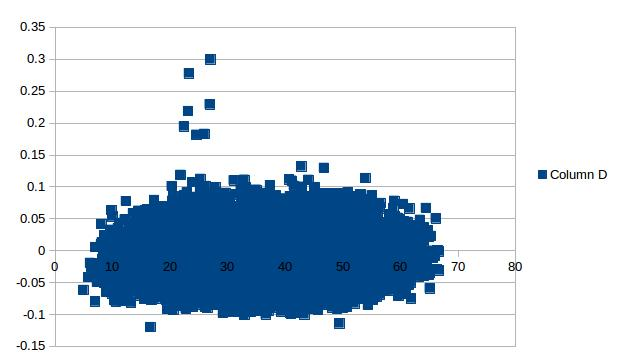
\includegraphics[scale=0.4]{3a0r_plmdca.jpg}
\caption{X axis: 3D distance in Anstrom. Y axis: DCA score}
\label{3d_dca}
\end{figure}

\begin{figure}
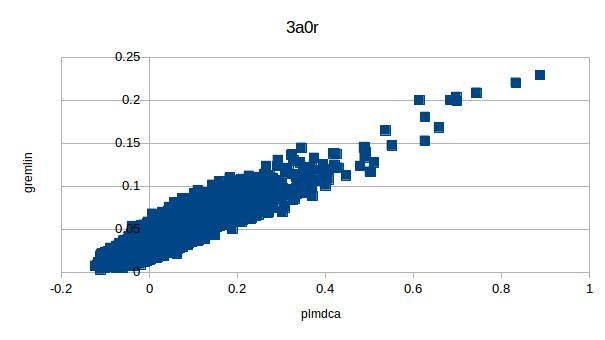
\includegraphics[scale=0.5]{3a0r_plmdca_gremlin.jpg}
\caption{X axis: DCA score. Y axis: Gremlin score}
\label{dca_gremlin}
\end{figure}





\section*{DCA based Approaches for Homodimer Proteins}
\end{document}